\de{ĐỀ THI HỌC KỲ I NĂM HỌC 2022-2023}{TRƯỜNG THPT Hai Bà Trưng - Huế}
\begin{center}
	\textbf{PHẦN 1 - TRẮC NGHIỆM}
\end{center}
\Opensolutionfile{ans}[ans/ans]


\begin{ex}%[0D1Y2-1]
	Cho tập hợp $A=\{x\in \mathbb{R} \mid x-3<0\}$. Tập hợp $A$ là tập nào sau đây?
	\choice
	{$A=[-\infty; 3)$}
	{$A=(3;+\infty)$}
	{\True $A=(-\infty; 3)$}
	{$A=(-\infty; 3]$}
	\loigiai{
		Ta có $x-3<0 \Leftrightarrow x<3$, suy ra $A=(-\infty; 3)$.
	}
\end{ex}

\begin{ex}%[0D1B3-2]
	Cho tập hợp $E=\{2n \mid n\in \mathbb{N}, n<5\}$ và $F=\left\{x\in \mathbb{R} \mid x^{2}-10x+24=0\right\}$. Trong các khẳng định sau, khẳng định nào đúng?
	\choice
	{$E \cap F=\{0; 4; 6\}$}
	{$C_{E} F=\{4; 6\}$}
	{\True $C_{E} F=\{0; 2; 8\}$}
	{$E \cap F=\{2; 6\}$}
	\loigiai{
		Ta có $E=\{0; 2; 4; 6; 8\}$ và $F=\{4; 6\}$ suy ra $C_{E} F=\{0; 2; 8\}$.
	}
\end{ex}

\begin{ex}%[0H2B2-5]
	Cho tam giác $ABC$ vuông tại $A$ có $BC=16$. Tính độ dài của véc-tơ $\overrightarrow{AB}+\overrightarrow{AC}$.
	\choice
	{$4$}
	{$4\sqrt{3}$}
	{\True $16$}
	{$8$}
	\loigiai{
		Gọi $M$ là trung điểm của $BC$.\\
		Ta có $\left|\overrightarrow{AB}+\overrightarrow{AC}\right|=\left|2\overrightarrow{AM}\right|=2AM=BC=16$.
	}
\end{ex}

\begin{ex}%[0D2B2-2]
	\immini
	{Miền nghiệm của hệ bất phương trình $\heva{&x+2y-100 \leq 0\\&2x+y-80 \leq 0\\&x \geq 0\\&y \geq 0}$ là miền đa giác (phần tô đậm) như hình. Tìm giá trị lớn nhất của biểu thức $F(x; y)=4x+3y$ với $(x; y)$ thỏa mãn hệ bất phương trình đã cho.
	\choice
	{$160$}
	{$150$}
	{\True $200$}
	{$220$}}
	{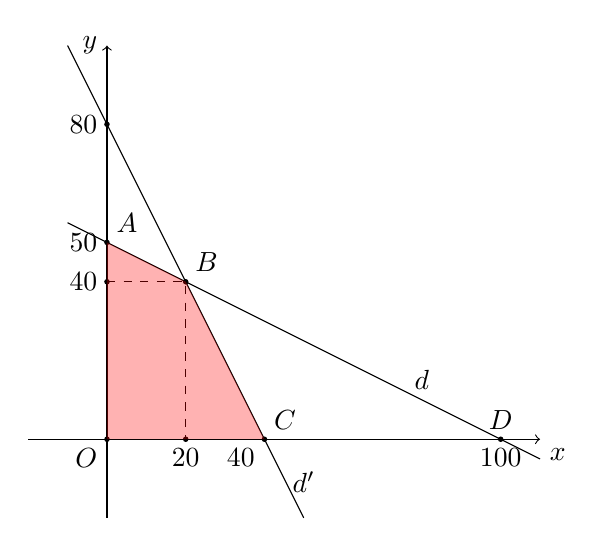
\begin{tikzpicture}[x=1cm,y=1cm,scale=1]
			\draw[->] (-1,0)--(5.5,0)node[below right]{$x$};
			\draw[->] (0,-1)--(0,5)node[left]{$y$};
			\fill (0,0)node[below left]{$O$}circle(1pt);
			\path (0,2.5)coordinate[label=above right:$A$](A) (1,2)coordinate[label=above right:$B$](B) (2,0)coordinate[label=above right:$C$](C) (5,0)coordinate[label=above:$D$](D) (0,4)coordinate[label=left:$80$](M) (0,2)coordinate[label=left:$40$](N) (1,0)coordinate[label=below:$20$](P) (0,2.5)coordinate[label=left:$50$]() (5,0)coordinate[label=below:$100$]() (2,0)coordinate[label=below left:$40$];
			\fill (4,1)node[below]{$d$};
			\fill (2.5,-0.8)node[above]{$d'$};
			\draw[black,samples=150,smooth,domain=-0.5:2.5] plot(\x,{-2*(\x)+4});
			\draw[black,samples=150,smooth,domain=-0.5:5.5] plot(\x,{-1/2*(\x)+2.5});
			\draw[dashed] (0,2)--(1,2)--(1,0);
			\foreach \diem in {A,B,C,D,M,N,P} \fill[black](\diem)circle(1pt);
			\fill[red,opacity=0.3] (0,2.5)--(1,2)--(2,0)--(0,0)--(0,2.5);
	\end{tikzpicture}}
	\loigiai{
		Ta có $A(0;50)$, $B(20;40)$, $C(40;0)$.\\
		Khi đó $F(0;0)=0$, $F(0;50)=150$, $F(20;40)=200$, $F(40;0)=160$.\\
		Vậy $\max F(x;y)=F(20;40)=200$.
	}
\end{ex}

\begin{ex}% [0H2Y2-3]
	Cho tam giác $ABC$ có $M$ là trung điểm của $BC$. Trong các khẳng định sau, khẳng định nào đúng?
	\choice
	{$\overrightarrow{MA}+\overrightarrow{MB}=\overrightarrow{MC}$}
	{$\overrightarrow{AB}+\overrightarrow{AC}=\overrightarrow{AM}$}
	{$\overrightarrow{MB}+\overrightarrow{MC}=\overrightarrow{BC}$}
	{\True $\overrightarrow{MB}+\overrightarrow{MC}=\overrightarrow{0}$}
	\loigiai{
		Có $M$ là trung điểm của $BC$ suy ra $\overrightarrow{MB}+\overrightarrow{MC}=\overrightarrow{0}$.
	}
\end{ex}

\begin{ex}%[0X1Y1-3]
	Hãy viết số quy tròn của số gần đúng $a=10658$ đến hàng trăm.
	\choice
	{$10650$}
	{$10600$}
	{$10660$}
	{\True $10700$}
	\loigiai{
		Số quy tròn của số gần đúng $a=10658$ đến hàng trăm là $10700$.
	}
\end{ex}

\begin{ex}% [0H1Y2-2]
	Cho tam giác $ABC$ với $BC=a$, $AC=b$, $AB=c$. Gọi $R$, $r$, $p$, $S$ lần lượt là bán kính đường tròn ngoại tiếp, bán kính đường tròn nội tiếp, nửa chu vi và diện tích của tam giác $ABC$. Trong các khẳng định sau đây có bao nhiêu khẳng định \textbf{sai}?\\
	(I). $S=\dfrac{1}{2} ab \sin C$.\\
	(II). $\dfrac{a}{\sin A}=2R$.\\
	(III). $a^{2}=b^{2}+c^{2}+2bc \cdot \cos A$.\\
	(IV). $S=pr$.\\
	\choice
	{$1$}
	{\True $3$}
	{$2$}
	{$0$} 
	\loigiai{
		Các khẳng định đúng là $S=\dfrac{1}{2} ab \sin C$; $\dfrac{a}{\sin A}=2R$; $S=pr$.
	}
\end{ex}

\begin{ex}%[0H2Y3-1]
	Cho $\vec{b}=2\vec{a}$ và $|\vec{a}|=4$. Tính độ dài của véc-tơ $\vec{b}$.
	\choice
	{$|\vec{b}|=4$}
	{$|\vec{b}|=6$}
	{$|\vec{b}|=2$}
	{\True $|\vec{b}|=8$}
	\loigiai{
		Ta có $|\vec{b}|=|2\vec{a}|=2|\vec{a}|=2\cdot 4=8$.
	}
\end{ex}

\begin{ex}%[0H1B2-1] 
	Cho tam giác có độ dài ba cạnh lần lượt là $4$; $5$; $6$. Tính cosin của góc có số đo nhỏ nhất của tam giác.
	\choice
	{$\dfrac{1}{8}$}
	{\True $\dfrac{3}{4}$}
	{$\dfrac{9}{16}$}
	{$\dfrac{77}{60}$}
	\loigiai{
		Ta có $\cos \alpha = \dfrac{5^2+6^2-4^2}{2\cdot 5\cdot 6}=\dfrac{3}{4}$.
	}
\end{ex}

\begin{ex}%[0H1Y1-3]
	Cho hai góc $\alpha$, $\beta$ thỏa mãn $\alpha+\beta=180^{\circ}$. Tính giá trị của biểu thức $\cos \beta \cos \alpha-\sin \alpha \sin \beta$.
	\choice
	{$1$}
	{$2$}
	{$0$}
	{\True $-1$}
	\loigiai{
		Ta có $\alpha+\beta=180^{\circ}$ suy ra $\cos \beta=-\cos \alpha$; $\sin \beta=\sin \alpha$.\\
		Do đó $\cos \beta \cos \alpha-\sin \alpha \sin \beta=-\cos^2 \alpha - \sin^2 \alpha=-\left(\sin^2 \alpha + \cos^2 \alpha\right)=-1$.
	}
\end{ex}

\begin{ex}%[0H1Y2-1]
	Cho tam giác $ABC$ với $BC=a$, $AC=b$, $AB=c$. Trong các khẳng định sau, khẳng định nào đúng?
	\choice
	{\True $\cos A=\dfrac{b^{2}+c^{2}-a^{2}}{2bc}$}
	{$\cos A=\dfrac{a^{2}+c^{2}-b^{2}}{2ac}$}
	{$\cos A=\dfrac{b^{2}+a^{2}-c^{2}}{2ba}$}
	{$\cos A=\dfrac{b^{2}+c^{2}-a^{2}}{2}$}
	\loigiai{
		Ta có $\cos A=\dfrac{b^{2}+c^{2}-a^{2}}{2bc}$.
	}
\end{ex}

\begin{ex}% [0H1B2-2]
	Cho tam giác $ABC$ có $AB=2$, $AC=\sqrt{7}$, $\widehat{B}=60^{\circ}$. Tính diện tích của tam giác $ABC$.
	\choice
	{$\dfrac{\sqrt{3}}{2}$}
	{\True $\dfrac{3\sqrt{3}}{2}$}
	{$\dfrac{\sqrt{21}}{2}$}
	{$3\sqrt{3}$}
	\loigiai{
		Ta có $AC^2=AB^2+BC^2-2\cdot AB\cdot BC\cdot \cos \widehat{B} \Rightarrow BC^2-2BC-3=0 \Rightarrow BC=3$.\\
		Suy ra $S_{ABC}=\dfrac{1}{2}\cdot AB\cdot BC\cdot \sin \widehat{B}=\dfrac{1}{2}\cdot 2\cdot 3\cdot \sin 60^{\circ}=\dfrac{3\sqrt{3}}{2}$.
	}
\end{ex}

\begin{ex}%[0D2Y1-1]
	Trong các bất phương trình sau, bất phương trình nào là bất phương trình bậc nhất hai ẩn?
	\choice
	{$x^{2}+2x>0$}
	{\True $2x+3y<2$}
	{$2x^{2}-y>1$}
	{$x-y+2z \leq 20$}
	\loigiai{
		Bất phương trình $2x+3y<2$ là bất phương trình bậc nhất hai ẩn.
	}
\end{ex}

\begin{ex}%[0D2Y2-2]
	Điểm $O(0; 0)$ thuộc miền nghiệm của hệ bất phương trình nào sau đây?
	\choice
	{$\heva{&x+2y-1>0\\&3x+2y+3<0}$}
	{$\heva{&x+2y-1>0\\&3x+2y+3 \geq 0}$}
	{\True $\heva{&x+2y-1<0\\&3x+2y+3>0}$}
	{$\heva{&x+2y-1<0\\&3x+2y+3<0}$}
	\loigiai{
		Điểm $O(0; 0)$ thuộc miền nghiệm của hệ bất phương trình $\heva{&x+2y-1<0\\&3x+2y+3>0.}$
	}
\end{ex}

\begin{ex}%[0D2B2-2]
	Miền nghiệm của hệ bất phương trình $\heva{&x \geq 1\\&x+y \leq 2\\&y \geq 0}$ là
	\choice
	{Miền tứ giác}
	{Miền tam giác}
	{Miền ngũ giác}
	{Một nửa mặt phẳng}
	\loigiai{
		\immini
		{Miền nghiệm của hệ bất phương trình $\heva{&x \geq 1\\&x+y \leq 2\\&y \geq 0}$ là miền tam giác.}
		{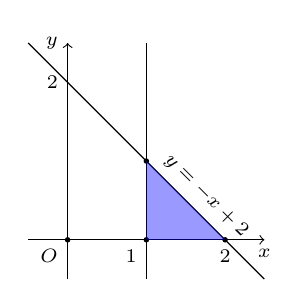
\begin{tikzpicture}[x=1cm,y=1cm,scale=1,font=\scriptsize]
				\draw[->] (-0.5,0)--(2.5,0)node[below]{$x$};
				\draw[->] (0,-0.5)--(0,2.5)node[left]{$y$};
				\fill (0,0)node[below left]{$O$} circle(1pt);
				\fill (1,0)node[below left]{$1$} circle(1pt);
				\fill (0,2)node[left]{$2$};
				\fill (2,0)node[below]{$2$} circle(1pt);
				\fill (1,1) circle(1pt);
				\draw[black,samples=150,smooth,domain=-0.5:2.5] plot(\x,{-(\x)+2});
				\path (2,0)--(0,2) node[pos=.2,sloped,above,black]{$y=-x+2$};
				\draw (1,-0.5)--(1,2.5);
				\fill[blue,opacity=0.4] (1,0)--(2,0)--(1,1)--(1,0);
		\end{tikzpicture}}
	}
\end{ex}

\begin{ex}%[0H2B3-5]
	Cho tam giác $ABC$ có $G$ là trọng tâm. Trong các khẳng định sau, khẳng định nào \textbf{sai}?
	\choice
	{\True $\overrightarrow{GA}=\overrightarrow{GB}+\overrightarrow{GC}$}
	{$|\overrightarrow{GA}+\overrightarrow{GB}+\overrightarrow{GC}|=0$}
	{$\overrightarrow{OA}+\overrightarrow{OB}+\overrightarrow{OC}=3\overrightarrow{OG}$, (với $O$ bất kỳ)}
	{$\overrightarrow{GA}+\overrightarrow{GB}+\overrightarrow{GC}=\overrightarrow{0}$}
	\loigiai{
		Khẳng định $\overrightarrow{GA}=\overrightarrow{GB}+\overrightarrow{GC}$ là sai.
	}
\end{ex}

\begin{ex}%[0H1Y1-2]
	Trong các khẳng định sau, khẳng định nào \textbf{sai}?
	\choice
	{$\tan 135^{\circ}=-1$}
	{\True $\sin 135^{\circ}=\dfrac{-\sqrt{2}}{2}$}
	{$\cot 135^{\circ}=-1$}
	{$\cos 135^{\circ}=\dfrac{-\sqrt{2}}{2}$}
	\loigiai{
		Khẳng định $\sin 135^{\circ}=\dfrac{-\sqrt{2}}{2}$ là sai.
	}
\end{ex}

\begin{ex}%[0H3B2-4]
	Trong mặt phẳng $Oxy$, cho hai điểm $A(2; 1)$ và $B(-4; 3)$. Gọi $M$ là điểm có tung độ gấp đôi hoành độ sao cho $\triangle AMB$ vuông tại $A$. Giả sử $m$ là hoành độ của điểm $M$. Trong các khẳng định sau, khẳng định nào đúng?
	\choice
	{$m\in (-7;-3)$}
	{$m\in (-11;-7)$}
	{\True $m\in (2; 6)$}
	{$m\in (-3; 2)$}
	\loigiai{
		Gọi $M(m; 2m)$.\\
		Ta có $\overrightarrow{AB}=(-6;2)$, $\overrightarrow{AM}=(m-2; 2m-1)$.\\
		$\triangle AMB$ vuông tại $A$ khi $0=\overrightarrow{AB}\cdot \overrightarrow{AM}=-6(m-2)+2(2m-1)=-2m+10 \Leftrightarrow m=5$.
	}
\end{ex}


\begin{ex}%[0T6Y4-1]%[Dự án đề kiểm tra HKII NH22-23- Nguyễn Sĩ Đạt]%[Hai Bà Trưng]
Một học sinh có điểm trung bình môn học kì I cuả 7 môn học được cho trong bảng sau.
\begin{center}
\renewcommand\arraystretch{1.5}
\begin{tabular}{|>{\raggedright\arraybackslash}m{1.2cm} |>{\centering\arraybackslash}m{1.6cm}|>{\centering\arraybackslash}m{1.6cm}|>{\centering\arraybackslash}m{1.6cm}|>{\centering\arraybackslash}m{1.6cm}|>{\centering\arraybackslash}m{1.7cm}|>{\centering\arraybackslash}m{1.6cm}|>{\centering\arraybackslash}m{2cm}|}
\hline
\textbf{Môn} &Toán & Vật lí&Hóa học&Sinh học&Ngữ văn & Lịch sử&Tiếng Anh\\ 
\hline
\textbf{Điểm}&$8{,}6$ &$7{,}6$&$6{,}7$&$8{,}2$&$7{,}0$&$8{,}5$&$6{,}8$\\
\hline 
\end{tabular}
\end{center}
Khoảng biến thiên của bảng điểm trên là
\choice
{$1{,}7$}
{$2$}
{\True $1{,}9$}
{$1{,}8$}
\loigiai{
Sắp xếp mẫu số liệu theo thứ tự không giảm, ta có
$$6{,}7\quad 6{,}8\quad 7{,}0\quad 7{,}6\quad 8{,}2\quad 8{,}5\quad 8{,}6.$$
Khi đó khoảng biến thiên của mẫu số liệu là $R=8{,}6-6{,}7=1{,}9$.
}
\end{ex}

\begin{ex}%[0T1Y1-4]%[Dự án đề kiểm tra HKII NH22-23- Nguyễn Sĩ Đạt]%[Hai Bà Trưng]
Cho hai mệnh đề $P$ và $Q$. Điều kiện để mệnh đề $P\Rightarrow Q$ là mệnh đề \textbf{sai} là
\choice
{$P$ sai và $Q$ sai}
{$P$ sai và $Q$ đúng}
{$P$ đúng và $Q$ đúng}
{\True $P$ đúng và $Q$ sai}
\loigiai{Điều kiện để mệnh đề $P\Rightarrow Q$ là mệnh đề sai là $P$ đúng và $Q$ sai.}
\end{ex}

\begin{ex}%[0T5Y2-1]%[Dự án đề kiểm tra HKII NH22-23- Nguyễn Sĩ Đạt]%[Hai Bà Trưng]
Cho $5$ điểm $A$, $B$, $C$, $D$, $E$ bất kỳ. Trong các khẳng định sau, khẳng định nào đúng?
\choice
{\True $\vec{AB}+\vec{CD}+\vec{BC}-\vec{ED}=\vec{AE}$}
{$\vec{AB}+\vec{CD}+\vec{BC}-\vec{ED}=\vec{AB}$}
{$\vec{AB}+\vec{CD}+\vec{BC}-\vec{ED}=\vec{CE}$}
{$\vec{AB}+\vec{CD}+\vec{BC}-\vec{ED}=\vec{AC}$}
\loigiai{
Ta có $\vec{AB}+\vec{CD}+\vec{BC}-\vec{ED}=\left( \vec{AB}+\vec{BC}\right) +\left( \vec{CD}-\vec{ED}\right) =\vec{AC}+\vec{CE}=\vec{AE}$.
}
\end{ex}

\begin{ex}%[0T1B1-4]%[Dự án đề kiểm tra HKII NH22-23- Nguyễn Sĩ Đạt]%[Hai Bà Trưng]
Trong các mệnh đề sau, mệnh đề nào có mệnh đề đảo đúng?
\choice
{Nếu số nguyên $n$ có chữ số tận cùng là $0$ thì số nguyên $n$ chia hết cho $5$}
{\True Nếu tứ giác $ABCD$ có hai đường chéo cắt nhau tại trung điểm mỗi đường thì tứ giác $ABCD$ là hình chữ nhật}
{Nếu tứ giác $ABCD$ là hình chữ nhật thì tứ giác $ABCD$ có hai đường chéo bằng nhau}
{Nếu tứ giác $ABCD$ là hình thoi thì tứ giác $ABCD$ có hai đường chéo vuông góc với nhau}
\loigiai{
Xét mệnh đề \lq\lq Nếu tứ giác $ABCD$ có hai đường chéo cắt nhau tại trung điểm mỗi đường thì tứ giác $ABCD$ là hình chữ nhật\rq\rq\ có mệnh đề đảo là \lq\lq Nếu tứ giác $ABCD$ là hình chữ nhật thì hai đường chéo cắt nhau tại trung điểm của mỗi đường\rq\rq. Mệnh đề này đúng do tính chất của hình chữ nhật.
}
\end{ex}

\begin{ex}%[0T2Y1-2]%[Dự án đề kiểm tra HKII NH22-23- Nguyễn Sĩ Đạt]%[Hai Bà Trưng]
Trong các cặp số sau đây, cặp số nào \textbf{không phải} là nghiệm của bất phương trình $x-2y<1$ ?
\choice
{ $(-2 ; 1)$}
{\True $(1 ; 0)$}
{ $(-3 ;-1)$}
{ $(0 ; 1)$}
\loigiai{Thay $x=1$, $y=0$ vào bất phương trình $x-2y<1$, ta được $1-2\cdot 0<1$ là mệnh đề sai nên cặp số $(1 ; 0)$ không phải là nghiệm của bất phương trình đã cho.
}
\end{ex}

\begin{ex}%[0T1B2-1]%[Dự án đề kiểm tra HKII NH22-23- Nguyễn Sĩ Đạt]%[Hai Bà Trưng]
 Cho tập hợp $A=\left\{x \in \mathbb{Z} \mid 3 x^2-8 x+4=0\right\}$. HTập hợp $A$ có số phần tử là
\choice
{ $0$}
{ $2$}
{ Vô số}
{\True $1$}
\loigiai{Ta có $A=\left\{x \in \mathbb{Z} \mid 3 x^2-8 x+4=0\right\}=\left\{2\right\}$.\\
Vậy tập hợp $A$ có $1$ phần tử.
}
\end{ex}

\begin{ex}%[0T9Y1-1]%[Dự án đề kiểm tra HKII NH22-23- Nguyễn Sĩ Đạt]%[Hai Bà Trưng]
Trong mặt phẳng tọa độ $Oxy$, cho hai điểm $A(4;1)$, $B(-2;3)$. Tọa độ của vec-tơ $\vec{u}=\vec{OA}+\vec{OB}$ là
\choice
{\True $\vec{u}=(2;4)$}
{$\vec{u}=(1;2)$}
{$\vec{u}=(-6;2)$}
{$\vec{u}=(6;-2)$}
\loigiai{
Ta có $\vec{OA}=(4;1)$, $\vec{OB}=(-2;3)$. Khi đó $\vec{u}=\vec{OA}+\vec{OB}=(2;4)$. \\
}
\end{ex}

\begin{ex}%[0T9B1-3]%[Dự án đề kiểm tra HKII NH22-23- Nguyễn Sĩ Đạt]%[Hai Bà Trưng]
Trong mặt phẳng tọa độ $Oxy$, cho hình bình hành $ABCD$ có $A(2;3)$, $B(5;1)$ và điểm $C$ nằm trên trục $Ox$, điểm $D$ nằm trên trục $Oy$. Tâm của hình bình hành $ABCD$ là $I(m;n)$. Giá trị của tổng $S=m+n$ là
\choice
{\True $4$}
{$8$}
{$2$}
{$6$}
\loigiai{
Gọi tọa độ của điểm $C(c;0)$ và $D(0;d)$.\\
Ta có $\vec{AB}=(3;-2)$, $\vec{DC}=(c;-d)$.\\
Vì $ABCD$ là hình bình hành nên 
$\vec{AB}=\vec{DC}
\Leftrightarrow \heva{&3=c\\&-2=-d}
\Leftrightarrow \heva{&c=3\\&d=2.}$\\
Ta có $I$ là tâm của hình bình hành $ABCD$ nên $I$ là trung điểm của $AC$, khi đó 
$$\heva{&x_I=\dfrac{x_A+x_C}{2}\\&y_I=\dfrac{y_A+y_C}{2}}
\Leftrightarrow \heva{&x_I=\dfrac{2+3}{2}=\dfrac{5}{2}\\&y_I=\dfrac{3+0}{2}=\dfrac{3}{2}}
\Leftrightarrow \heva{&m=\dfrac{5}{2}\\&n=\dfrac{3}{2}.}$$
Vậy $S=m+n=\dfrac{5}{2}+\dfrac{3}{2}=4$.
}
\end{ex}

\begin{ex}%[0T4B2-1]%[Dự án đề kiểm tra HKII NH22-23- Nguyễn Sĩ Đạt]%[Hai Bà Trưng]
Cho tam giác $ABC$ có $AB=5$, $\widehat{B}=75^\circ$, $\widehat{A}=45^\circ$. Bán kính đường tròn ngoại tiếp tam giác $ABC$ là
\choice
{$10$}
{$5 \sqrt{2}$}
{\True $\dfrac{5\sqrt{3}}{3}$}
{$\dfrac{10\sqrt{3}}{3}$}
\loigiai{
Ta có $\widehat{C}=180^\circ -\widehat{B}-\widehat{A}=180^\circ -75^\circ-45^\circ = 60^\circ $.\\
Áp dụng định lí sin, ta có 
$2R=\dfrac{AB}{\sin C}=\dfrac{5}{\sin 60^\circ}=\dfrac{10\sqrt{3}}{3}\Leftrightarrow R=\dfrac{5\sqrt{3}}{3}$. \\
Vậy bán kính cần tìm là $\dfrac{5\sqrt{3}}{3}$.
}
\end{ex}

\begin{ex}%[0T5B4-1]%[Dự án đề kiểm tra HKII NH22-23- Nguyễn Sĩ Đạt]%[Hai Bà Trưng]
Cho hình vuông $ABCD$ có cạnh bằng $4$. Tính $\vec{AB} \cdot \vec{AC}$.
\choice
{\True$16$}
{$-16$}
{$8 \sqrt{2}$}
{$-8 \sqrt{2}$}
\loigiai{
Ta có $\vec{AB} \cdot \vec{AC}=AB \cdot AC \cdot \cos (\vec{AB} , \vec{AC})= AB \cdot AC \cdot \cos \widehat{BAC}= 4\cdot 4 \cos 45^\circ = 8 \sqrt{2}$.
}
\end{ex}

\begin{ex}%[0T4Y1-2]%[Dự án đề kiểm tra HKII NH22-23- Nguyễn Sĩ Đạt]%[Hai Bà Trưng]
Cho góc $\alpha\,\, (0^\circ < \alpha < 90^\circ)$. Trong các khẳng định sau, khẳng định nào \textbf{sai}? 
\choice
{\True $\tan(90^\circ - \alpha) = -\cot\alpha$}
{$\cos(90^\circ - \alpha) = \sin\alpha$}
{$\cot(90^\circ - \alpha) = \tan\alpha$}
{$\sin(90^\circ - \alpha) = \cos\alpha$}
\loigiai{
Ta có $\tan(90^\circ - \alpha) = \cot\alpha$ nên khẳng định $\tan(90^\circ - \alpha) = -\cot\alpha$ là sai.
}
\end{ex}

\begin{ex}%[0T5B1-3]%[Dự án đề kiểm tra HKII NH22-23- Nguyễn Sĩ Đạt]%[Hai Bà Trưng]
Cho hình vuông $ABCD$ có cạnh bằng $a$. Giá trị  $\left|\vec{AB}+2\vec{AD}\right|$ theo $a$ là
\choice
{$3a$}
{\True $a\sqrt{5}$}
{$a\sqrt{3}$}
{$a\sqrt{2}$}
\loigiai{
Lấy điểm $M$ sao cho $\vec{AM}=2\vec{AD}$ như hình vẽ.
\begin{center}
\begin{tikzpicture}[>=stealth]
\coordinate[label=left:{$D$}] (D) at (-4,0);
\coordinate[label=right:{$C$}] (C) at (0,0);
\coordinate[label=below:{$M$}] (M) at (-4,-4);
\coordinate[label=left:{$A$}] (A) at (-4,4);
\coordinate[label=right:{$B$}] (B) at (0,4);
\draw[black] (B)--(M) (D)--(A)--(B)--(C)--(D)--(M)  ;
\foreach \diem in {A,B,C,D,M}\fill[black] (\diem)circle(1.5pt);
\end{tikzpicture}
\end{center}
Khi đó $\left|\vec{AB}+2\vec{AD}\right| =\left| \vec{AB}+\vec{AM}\right| =\left| \vec{BM}\right| =\sqrt{a^2+(2a)^2}=a\sqrt{5}$.
}
\end{ex}

\begin{ex}%[0T5Y1-3]%[Dự án đề kiểm tra HKII NH22-23- Nguyễn Sĩ Đạt]%[Hai Bà Trưng]
Cho hình chữ nhật $ABCD$. Trong các khẳng định sau, khẳng định nào đúng?
\choice
{$\overrightarrow{AB}$ và $\overrightarrow{AC}$ cùng phương}
{$\overrightarrow{AB}=\overrightarrow{CD}$}
{$\overrightarrow{AB}=\overrightarrow{CD}$}
{\True $\left| \overrightarrow{AC}\right| =\left| \overrightarrow{BD}\right|$}
\loigiai{
Do $ABCD$ là hình chữ nhật nên $ \left| \overrightarrow{AC}\right| =\left| \overrightarrow{BD}\right| $.
}
\end{ex}

\begin{ex}%[0T6Y3-3]%[Dự án đề kiểm tra HKII NH22-23- Nguyễn Sĩ Đạt]%[Hai Bà Trưng]
Bảng số liệu dưới đây cho biết số áo sơ mi nam bán được trong một tháng của một cửa hàng.
\begin{center}
\begin{tabular}{|l|c|c|c|c|c|c|c|}
\hline
Cỡ áo & 36 & 37 & 38 & 39 & 40 & 41 & 42\\
\hline
Số áo bán được & 7 & 15 & 20 & 28 & 20 & 13 & 8\\
\hline
\end{tabular}
\end{center}
Mốt của bảng số liệu trên la
\choice
{\True$39$}
{$38$}
{$28$}
{$42$}
\loigiai{Ta thấy cỡ áo $39$ bán được nhiều nhất ($28$ cái). Do đó, mốt của bảng số liệu là $39$.
}
\end{ex}

\begin{ex}%[0T6B3-1]%[Dự án đề kiểm tra HKII NH22-23- Nguyễn Sĩ Đạt]%[Hai Bà Trưng]
Điểm kiểm tra môn Toán của $47$ học sinh được cho trong bảng dưới đây.
\begin{center}
\begin{tabular}{|l|c|c|c|c|c|c|c|c|c|c|c|}
\hline
Điểm& $0$& $1$ & $2$ & $3$ & $4$ & $5$ & $6$ & $7$ & $8$ & $9$ & $10$\\
\hline
Số học sinh& 0 & 0 & 0 & 1 & 2 & 8 & 9 & 11 & 8 & 6 & 2 \\
\hline
\end{tabular}
\end{center}
Tính điểm kiểm tra trung bình môn Toán của $47$ học sinh trên (làm tròn kết quả đến hàng phần chục).
\choice
{\True$6{,}8$}
{ $6{,}9$}
{$7$}
{$6{,}7$}
\loigiai{
Điểm kiểm tra trung bình môn Toán của $47$ học sinh trên là
\begin{center}
$\overline{x}=\dfrac{0\cdot0+1\cdot0+2\cdot0+3\cdot1+4\cdot2+5\cdot8+6\cdot9+7\cdot11+8\cdot8+9\cdot6+10\cdot2}{47}\approx{6{,}8}$ (điểm).
\end{center}
}
\end{ex}

\begin{ex}%[0T5Y4-1]%[Dự án đề kiểm tra HKII NH22-23- Nguyễn Sĩ Đạt]%[Hai Bà Trưng]
Cho hai vec-tơ $\vec{u}\cdot \vec{v}$ khác vec-tơ-không. Trong các khẳng định sau, khẳng định nào \textbf{đúng}?
\choice
{$\vec{u}\cdot \vec{v}=\left|\vec{u}\right|\cdot \left|\vec{v}\right|$}
{$\left|\vec{u}\right|\cdot \left|\vec{v}\right|=\vec{u}\cdot \vec{v}\cdot \cos \left(\vec{u},\vec{v}\right)$}
{$\vec{u}\cdot \vec{v}=\left|\vec{u}\right|\cdot \left|\vec{v}\right|\cdot \sin \left(\vec{u},\vec{v} \right)$}
{\True $\vec{u}\cdot \vec{v}=\left|\vec{u}\right|\cdot \left|\vec{v}\right|\cdot \cos \left(\vec{u},\vec{v} \right)$}
\loigiai{Công thức tính tích vô hướng của hai vec-tơ là $\vec{u}\cdot \vec{v}=\left|\vec{u}\right|\cdot \left|\vec{v}\right|\cdot \cos \left(\vec{u},\vec{v} \right)$.}
\end{ex}

\begin{ex}%[0T6Y1-1]%[Dự án đề kiểm tra HKII NH22-23- Nguyễn Sĩ Đạt]%[Hai Bà Trưng]
Đo độ cao của một ngọn núi cho kết quả là $1380{,}5 \pm 0{,}2 $ m. Độ chính xác $d$ của phép đo trên là
\choice
{\True $d=0{,}2$ m}
{ $d=0{,}7$ m}
{ $d= \pm 0{,}2$ m}
{ $d= \pm 0{,}7$ m}
\loigiai{Độ chính xác $d$ là $0{,}2$ m.
}
\end{ex}

\Closesolutionfile{ans}
%\begin{center}
%\textbf{ĐÁP ÁN}
%\inputansbox{10}{ans/ans}
%\end{center}


\begin{center}
	\textbf{PHẦN 2 - TỰ LUẬN}
\end{center}






\begin{bt}%[0D1K3-4]%Câu 1%[Dự án đề kiểm tra HK1 NH22-2-Lê Hùng Thắng]%[THPT Hai Bà Trưng - Huế]
	Cho ba tập hợp $A=\{n \in \mathbb{N}\mid n \leq 2\}$, $B=\left\{x \in \mathbb{N}\mid x^2-5 x+6=0\right\}$ và $C=[m; m+3]$. Tìm tất cả các giá trị thực của tham số $m$ để $A \cap B \subset C$.
	\loigiai{
	Ta có $A=\{0;1;2\}$, $B=\{2;3\}$,  $A \cap B= \{2\}$.\\
	Do đó $A \cap B \subset C  \Leftrightarrow 2 \in C \Leftrightarrow \heva{&m \le 2\\& 2\le m+3}  \Leftrightarrow \heva{&m \le 2 \\& m \ge -1}  \Leftrightarrow -1 \le m \le 2$.
}
\end{bt}

\begin{bt}%[0H1B2-1]%Câu 2%[Dự án đề kiểm tra HK1 NH22-2-Lê Hùng Thắng]%[THPT Hai Bà Trưng - Huế]
	Cho tam giác $ABC$ có $b=8$, $c=5$, $\widehat{A}=60^{\circ}$. Tính bán kính của đường tròn nội tiếp tam giác $A B C$.
		\loigiai{
	Ta có $a^2=b^2+c^2=2\cdot b\cdot c\cos A = 64+25-2\cdot 8 \cdot 5 \cdot \cos 60^\circ = 49$.\\
	Suy ra $a=7$.\\
	Lại có $\dfrac{a}{\sin A}=2R  \Rightarrow R=\dfrac{a}{2 \sin A}=\dfrac{7}{2 \sin 60^\circ} = \dfrac{7 \sqrt{3}}{3}$.	
	}
\end{bt}

\begin{bt}%[0H1K2-2]%Câu 3%[Dự án đề kiểm tra HK1 NH22-2-Lê Hùng Thắng]%[THPT Hai Bà Trưng - Huế]	
	Cho tam giác $ABC$ thỏa mãn $S=\dfrac{1}{4}c^2 \tan B$. Chứng minh $\triangle A B C$ cân.
		\loigiai{
	Ta có $\dfrac{b}{\sin B}=2R \Rightarrow \sin B = \dfrac{b}{2R}$; $\cos B = \dfrac{a^2+c^2-b^2}{2ac}$.\\
	Suy ra $\tan B = \dfrac{\sin B}{\cos B}=\dfrac{b}{2R}\cdot \dfrac{2ac}{a^2+c^2-b^2}=\dfrac{abc}{R\cdot(a^2+c^2-b^2)}$.\\
	Theo đề, ta có 
	\allowdisplaybreaks \vspace*{-0.6cm}
	\begin{eqnarray*} 
		& & S=\dfrac{1}{4}c^2 \tan B \\
		& \Leftrightarrow & \dfrac{abc}{4R} = \dfrac{1}{4}c^2 \dfrac{abc}{R\cdot(a^2+c^2-b^2)}\\
		& \Leftrightarrow & c^2= a^2+c^2-b^2\\
		& \Leftrightarrow & a^2=b^2 \\
		& \Leftrightarrow & a=b.
	\end{eqnarray*}
Vậy tam giác $ABC$ cân tại $C$.
	}
\end{bt}

\begin{bt}%[0H3K1-4]%[0H3B1-3]%Câu 4%[Dự án đề kiểm tra HK1 NH22-2-Lê Hùng Thắng]%[THPT Hai Bà Trưng - Huế]
	Trong mặt phẳng $Oxy$, cho tam giác $ABC$ có $A(-1;5)$, $B(0;2)$, $C(6;0)$.
	\begin{enumEX}{1}
	\item Tìm tọa độ trung điểm $M$ của cạnh $B C$ và tính độ dài đường trung truyến $A M$ của tam giác $A B C$.
	\item Tìm tọa độ điểm $N$ trên trục $O x$ để ba điểm $A, M, N$ thẳng hàng.
	\end{enumEX}
	\loigiai{
	\begin{enumEX}{1}
	\item Trung điểm của $BC$ là $M(3;1)$.\\
	Ta có $\vec{AM}=(4;-4) \Rightarrow AM= \left|\vec{AM}\right|=\sqrt{4^2+(-4)^2}=4\sqrt{2}$.
	\item Gọi $N(x;0) \in Ox$.\\
	Ta có $\vec{AM}=(4;-4)$, $\vec{AN}=(x+1;-5)$.\\
	Ba điểm $A, M, N$ thẳng hàng khi $\vec{AM}$ và $\vec{AN}$ cùng phương\\
	$\Leftrightarrow 4\cdot (-5) = -4\cdot (x+1) \Leftrightarrow x=4$.\\
	Vậy $N(4;0)$.
\end{enumEX}	
}
\end{bt}

\begin{bt}%[0H2G3-6]%Câu 5%[Dự án đề kiểm tra HK1 NH22-2-Lê Hùng Thắng]%[THPT Hai Bà Trưng - Huế]
	Cho hình chữ nhật $ABCD$ có $AB=12$ và $AD=4$. Khi điểm $M$ thay đổi trên cạnh $CD$, tìm giá trị nhỏ nhất của biểu thức $T=\left| \vec{MA}+2 \vec{MB}+3 \vec{MC}\right|$.
	\loigiai{
\immini{
	Gọi $I$, $K$ lần lượt là trung điểm của $AC$, $BC$ và $G$ là trọng tâm tam giác $IBC$. Khi đó $G\in IK$.\\
	Ta có 
	\allowdisplaybreaks 
	$\begin{aligned}[t]
		&\, \vec{MA}+2 \vec{MB}+3 \vec{MC}\\
		= &\, \vec{MA}+\vec{MC}+2 \vec{MB}+2 \vec{MC} \\
		= &\, 2\vec{MI}+2 \vec{MB}+2 \vec{MC} \\
		= &\, 2(\vec{MI}+\vec{MB}+\vec{MC})\\
		= &\, 6\vec{MG}.
	\end{aligned}$\\
}
{\begin{tikzpicture}[scale=1,>=stealth, font=\footnotesize, line join=round, line cap=round]
		\path (0,0) coordinate (D)
		(0,2) coordinate (A)
		(6,2) coordinate (B)
		(6,0) coordinate (C)
		(2.5,0) coordinate (M)
		($(A)!0.5!(C)$) coordinate (I)
		($(B)!0.5!(C)$) coordinate (K)
		($(I)!2/3!(K)$) coordinate (G)
		($(C)!(G)!(D)$) coordinate (H);
\draw (A)--(B)--(C)--(D)--(A)--(C) (B)--(I)--(K)
(M)--(G)--(H);
\foreach \d/\g in {A/150,B/30,C/0,D/180,I/90,K/0,G/90,M/-90,H/-90} \fill (\d) circle (1pt) ++(\g:2.5mm) node {$\d$}; 
	\end{tikzpicture}
}	
\noindent 
$T=\left|\vec{MA}+2 \vec{MB}+3 \vec{MC}\right|=6\left|\vec{MG}\right|=6MG \ge 6HG =6CK$.\\
Với $H$ là hình chiếu của $G$ lên $CD$.\\
Do đó giá trị nhỏ nhất của $T$ là $T_0=6CK=3BC=12$.\\
}
\end{bt}



